\documentclass{article}

\usepackage[margin=0.5in]{geometry}
\usepackage{tikz}
\usepackage{tikz-qtree}

\title{Problem Set 2}
\author{Mark Xavier (xaviem01)}

\begin{document}
	
	\maketitle
	
	\begin{enumerate}
		\item Alpha-Beta Pruning - assuming we work left to right and we prune if we decide that a sub-tree is not worth reviewing:
		
		\begin{center}
			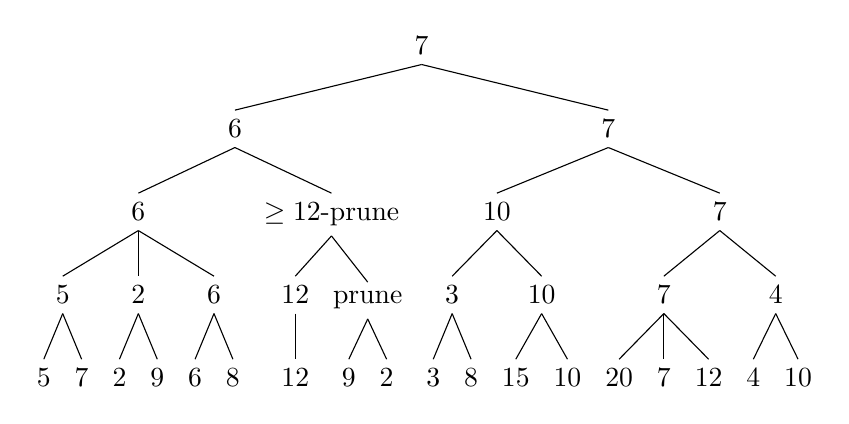
\begin{tikzpicture}
				\Tree[.7 [.6 
				             [.6 
				                 [.5 [.5 ] [.7 ]]  
				                 [.2 [.2 ] [.9 ] ] 
				                 [.6 [.6 ] [.8 ] ]] 
				             [.$\geq12$-prune 
				                 [.12 [.12 ] ] 
				                 [.prune [.9 ] [.2 ] ]]] 
						 [.7
						     [.10 
						         [.3 [.3 ] [.8 ] ] 
						         [.10 [.15 ] [.10 ]]] 
						     [.7
						         [.7 [.20 ] [.7 ] [.12 ]] 
						         [.4 [.4 ] [.10 ]]]] 
					 ]
			\end{tikzpicture}
		\end{center}
	
		I only encountered one area that could be pruned (the node $\geq 12$) - in this case the best move for MAX is to take the right side tree and get a score of 7 as opposed to 6.\\
		
		\item Convert the following to clausal form:\\
		2.1. $C \Rightarrow (A \Leftrightarrow B)$\\
		2.2. $(\neg C \vee E) \Rightarrow B$\\
		2.3. $D \Rightarrow \neg B$\\
		2.4. $(A \wedge D) \Rightarrow \neg E$\\
		2.5. $C \vee D \vee E$\\
		2.6. $E \Rightarrow D$
		
		Taking these one at a time (\textbf{NOTE: I use the equivalency symbol $\equiv$ between steps}):\\
		
		2.1. $C \Rightarrow (A \Leftrightarrow B) \equiv C \Rightarrow ((A \Rightarrow B) \wedge (B \Rightarrow A)) \equiv \neg C \vee ((\neg A \vee B) \wedge (\neg B \vee A)) \equiv (C \vee (\neg A \vee B)) \wedge (C \vee (\neg B \vee A))$
		
		Which breaks to:
		
		$C \vee \neg A \vee B\\
		 C \vee  \neg B \vee A$\\
		
		2.2. $(\neg C \vee E) \Rightarrow B \equiv \neg(\neg C \vee E) \vee B \equiv (\neg\neg C \wedge \neg E) \vee B \equiv (C \wedge \neg E) \vee B \equiv (C \vee B) \wedge (\neg E \vee B)$
		
		Which breaks into:
		
		$C \vee B\\
		\neg E \vee B$\\
		
		2.3. $D \Rightarrow \neg B \equiv \neg D \vee \neg B$, which is in clausal form.\\
		
		2.4. $(A \wedge D) \Rightarrow \neg E \equiv \neg(A \wedge D) \vee \neg E \equiv \neg A \vee \neg D \vee \neg E$, which is in clausal form.\\

		2.5. $C \vee D \vee E$ is already in clausal form.\\
		
		2.6. $E \Rightarrow D \equiv \neg E \vee D$, which is in clausal form.\\
		
		\item Davis-Putnam Algorithm on sentences in problem 2:\\
		
		3.1. This case is easy, given:
		
		$C \vee \neg A \vee B\\
		C \vee  \neg B \vee A$
		
		The first run of the loop finds the pure-literal $C$, and since it is not a negated $C$ it assigns the value TRUE to $C$, and then deletes all clauses containing $C$ from the set of clauses $S$, which deletes all clauses.  Then in the second run of the loop, since $S = \emptyset$, we assign TRUE or FALSE to B (if we always assign TRUE first then both are assigned TRUE), and we return $C=$TRUE, $A=$TRUE, and $B=$TRUE.\\
		
		3.2. Again, similar to problem 1, here we encounter the pure literal B (technically C and E are also pure literals, but alphabetically we'd hit B first), we assign $B=$TRUE, then delete both clauses.  In the next iteration of the loop we exit since $S = \emptyset$, and assign B, C, and E all TRUE.\\
		
		3.3. Depending on how this algorithm is written, this can go two ways.  Either $\neg B$ and $\neg D$ are both viewed as pure literals, $B$ is assigned FALSE, and then we end as we did in the previous two responses (with D=TRUE), or we assume there are no "easy" cases and we try random assignment.  In the latter case, we assign $B$ to TRUE then delete B from the clause, then we find that the remaining clause only contains the literal $\neg D$, so we run "obviousassign()" and assign D=FALSE, making the clause TRUE, then we run a third iteration, find that S is empty, and return B=TRUE and D=FALSE (this assumes we check atoms in alphabetical order).\\
		
		3.4. Just like in the previous answer, either $\neg A$ is considered a pure literal and is assigned FALSE, which makes the statement true and exits after the second iteration sees $S = \emptyset$, or $A$ and $D$ are assigned TRUE and removed from the clause, then $\neg E$ is found to be the only symbol remaining and E is appropriately assigned FALSE, making the entire statement true and returning.
		
		3.5. Similar to 3 and 4, C may be considered a pure literal off the bat and assigned TRUE (assigning TRUE to the other symbols as well) or we assume no "easy" cases and C is assigned TRUE arbitrarily.  On the second iteration of the loop, due to the propogation step, we find that $S$ is empty (as C=TRUE makes the clause itself TRUE), and we assign C=TRUE and the others as TRUE as well.
		
		3.6. Another case where we may terminate early finding that $\neg E$ or $D$ are pure literals (if done alphabetically we assign D=TRUE first, then E is arbitrarily assigned TRUE or FALSE) or we may arbitrarily assign the symbol D TRUE, then propogate which will find the statement itself true and remove it, leaving $S$ empty in the second iteration and returning D=TRUE and E=[TRUE or FALSE].
	\end{enumerate}
	
\end{document}